\documentclass{astroedu-lab}

\begin{document}

\pagestyle{plain}

\begin{problem}{\huge Лабораторная работа 3.7.3\\\\Длинные линии\\\\Выполнил Жданов Елисей Б01-205}

\section{Цель работы:}

Ознакомится и проверить на практике теорию распространения
электрических сигналов вдоль длинной линии; измерить амплитудо- и фазово-частотные
характеристики коаксиальной линии; определить погонные характеристики такой
линии; на примере модели длинной линии изучить вопрос распределения амплитуды
колебаний сигнала по длине линии.

\section{Оборудование:}

Осциллограф АКТАКОМ ADS-6142H; генератора АКИП 3420/1; бухта с
коаксиальным кабелем pk 50-4-11; схематический блок "модель длинной линии"; магазин
сопротивления Р33, соединительные провода

\section{Теоретическая справка}

Рассмотрим элемент dx длинного коаксиального кабеля. Этот элемент представляет собой изолированный коаксиальный проводящий (медный) цилиндр некоторого радиуса $r_2$, на оси которого расположен сплошной тонкий проводник (медный) круглого сечения с радиусом $r_1$. Пространство между этнми проводниками заполнена средой, обладающей диэлектрнческой проницаемостью $\varepsilon$ и магнитной воспринмчнвостыю $\mu$. Как нзвестно, такой элемент обладает нндуктнвностью
$$
d L=2 \mu \ln \left(r_2 / r_1\right) d x .
$$
Удельная (погонная) индуктнвность еднницы длнны такого кабеля:
$$
L_x=\frac{d L}{d x}=2 \mu \ln \left(r_2 / r_1\right) .
$$
Два проводника, образуюшнх этот элемент $d x$ коакснального кабеля, должны обладать взанмной ёмкостью. Можно показать, что ёмкость элемента $d x$ коаксиального кабеля опредегяется выражением:
$$
d C=\frac{\varepsilon}{2 \ln \left(r_2 / r_1\right)} d x,
$$
а его удельная (погонная) ёмкость единицы длнны равна:
$$
C_x=\frac{d C}{d x}=\frac{\varepsilon}{2 \ln \left(r_2 / r_1\right)} .
$$
Когда по такому кабелю передаётся сигнал, в его центральной жнле и внешней оболочке возникают взаимно противоположные токи $I(x)$, а также электрическое напряженне $U(x)$ между внешним и внутренним проводннкамн. При высоких тастотах $v$ сигналов, распространяющихся в кабеле (когда дннна кабеля $l>V / \nu$, где $V$ - характерная скорость распространения сигнала в кабеле, эта скорость, как правило, порядка скорости света) $I(x)$ и $U(x)$ вообще говоря зависят от коордннаты $x$.

Изменение напряжения на концах элемента $d x$ вызваны возникновением ЭДС индукцин и паденнем напряжения в результате омнческого сопротивления проводников:
$$
U(x+d x)-U(x)=-\frac{L_x d x}{c^2} \frac{\partial I}{\partial t}-R_x d x I,
$$
где погонное сопротивленне
$$
R_x=\frac{d R}{d x}=\frac{1}{\sigma \cdot S}
$$
здесь $\sigma$ - удельная проводнмость материала проводников, $S$ - площадь их поперечного сечения.

Измененне силы тока вызвано тем, что некоторая часть электрического заряда $q$ как бы "перетекает на "обкладкн" конденсатора, роль которьх играют проводннки коакснального кабеля:
$$
I(x+d x)-I(x)=-\frac{\partial q}{\partial t},
$$
где $q=C_x d x U$
Представим уравнения (5) и (7) в внде системы, опнсывающей распространение сигнала вдоль длинной лннни:
$$
\left\{\begin{array}{l}
U(x)=U(x+d x)+\frac{L_x d x}{c^2} \frac{\partial I}{\partial t}+R_x d x I, \\
I(x)=I(x+d x)+\frac{\partial q}{\partial t} .
\end{array}\right.
$$
Эту систему уравнений называют телеграфными уравнениями. Разделим оба уравнения на длнну элемента $d x$ и, воспользовавшнсь определеннем дифференциалов, перепишем (8) следующим образом
$$
\left\{\begin{array}{l}
\frac{\partial I}{\partial x}=-C_x \frac{\partial U}{\partial t} \\
\frac{\partial U}{\partial x}=-\frac{L_x}{c^2} \frac{\partial I}{\partial t}-R_x I
\end{array}\right.
$$
Из (9) выразим перекрёстные производные:
$$
\left\{\begin{array}{l}
\frac{\partial^2 I}{\partial x \partial t}=-C_x \frac{\partial^2 U}{\partial^2 t}, \\
\frac{\partial^2 U}{\partial x^2}=-\frac{L_x}{c^2} \frac{\partial^2 I}{\partial x \partial t}-R_x \frac{\partial I}{\partial x}
\end{array} .\right.
$$
Из (9) и (10) получаем волновое уравнение для напряжения $U(x)$
$$
\frac{\partial^2 U}{\partial x^2}=\frac{L_x C_x}{c^2} \frac{\partial^2 U}{\partial t^2}+R_x C_x \frac{\partial U}{\partial t} .
$$
Илн в каноническом виде:
$$
\frac{\partial^2 U}{\partial t^2}-V_\phi^2 \frac{\partial^2 U}{\partial x^2}+\gamma \frac{\partial U}{\partial t}=0,
$$
где введены следующие обозначения для фазовой скорости:
$$
V_\phi=\frac{c}{\sqrt{L_x C_x}},
$$
и декремента затухания:
$\gamma=R_x C_x V_\phi^2$.
(14)








Подставляя (2) и (4) в выражение для фазовой скорости (13), легко видеть, что, эта скорость нмеет тот же вид, как и скорость распространения обычньх электромагнитных волн в некоторой среде с диэлектрической проницаемостью $\varepsilon$ и магнитной воспрнимчивостью $\mu$ :
$$
V_\phi=\frac{c}{\sqrt{q l}}
$$
Решение (12) удобно искать в виде:
$$
U(x, t)=U_0 e^{-i a t e r} e^{(-\alpha+i k) x} .
$$
Из первого уравнения системы (9) легко установить характер изменения силы тока в длинной линии:
$$
I(x, t)=U_0 \frac{C_x \omega}{k+i \alpha} e^{-i a t} e^{(-\alpha+i k) x}
$$
Из (16) и (17) видно, что отношение силы тока и напряжения в длинной линии не зависят от времени и координаты. Это отношение называют волновым сопротивлением (импедансом):
$$
Z(\omega, k)=\frac{U(x, t)}{I(x, t)}=\frac{k+i \alpha}{C_x \omega} .
$$
В пределе малых затуханий $\alpha \ll \omega$
$$
Z(\omega, k) \approx \frac{k}{C_x \omega}=\frac{1}{C_x V_\phi}=\frac{1}{c} \sqrt{\frac{L_x}{C_x}} .
$$
Если в конце такую длинную лннню замкнуть на сопротивление
$$
R_0=\frac{1}{c} \sqrt{\frac{L_x}{C_x}},
$$
то бегущая вдоль длинной линни волна "будет воспринимать" нагрузку как бесконечное продолжение этой длинной линии. Другими словами, когда длинная линия подключена $\mathrm{k}$ нагрузке с сопротивлением $R_0$, отражённой волны не возникает. Во всех остальных случаях, когда $R \neq R_0$ (в том числе и в частных случаях незамкнутого конца, когда $R \rightarrow \infty$ и короткозамкнутой линни, когда $R=0$ ) возникает отражённая волна, описываемая выражением (сравни с (13)):
$U(x, t)=U_0 e^{-i e t} e^{-(\alpha+i k) x}$, которое также удовлетворяет решенню системы (9).
Подставляя (16) в (12) получаем характеристическое уравнение:
$$
-\omega^2-V_\phi^2(-\alpha+i k)^2-i \omega \gamma=0 .
$$
Или, разделяя действительную и мнимую части, приходим к системе:
$$
\left\{\begin{array}{l}
\omega^2=V_\phi^2\left(k^2-\alpha^2\right) \\
2 \alpha k V_\phi^2=\omega \gamma
\end{array}\right.
$$
Из (22) следует (в пределе мальх затуханий $\alpha \ll<$ ):
$$
\begin{aligned}
\alpha=\frac{\omega}{V_\phi} \sqrt{\frac{\sqrt{1+(\gamma / \omega)^2}-1}{2}} & \approx \frac{\omega}{V_\phi} \sqrt{\frac{\gamma^2}{4 \omega^2}}=\frac{\gamma}{2 V_\phi}=R_x C_x \frac{V_\phi}{2}, \\
k & =\frac{\omega}{V_\phi} .
\end{aligned}
$$
Таким образом, амплитуда напряжения на нагрузке (в конце длинной линин) будет иметь вид:
$$
U_\mu(t)=U_0 e^{-a l} e^{i l d} e^{-t a t} .
$$
При этом амплитуда колебаннй на согласованной нагрузке (в конце длинной линии) имеет вид:
$$
U_n=U_0 e^{-a d}
$$
и набег фазы сигнала на выходе (в конце длинной линии) относительно входного сигнала (вначале длннной линии) будет иметь вид:
$$
\Delta \varphi=k l .
$$
Так как модуль волнового вектора $k$ прямо пропорционален частоте сигнала $\omega$ (см. выражение (24)) следует понимать, что разность фазы $\Delta \varphi$ монотонно увеличивается с увеличеннем $\omega$.

Из (26) и (27) легко экспериментально определить декремент затухания $\alpha$ и волновое число $k$ для различных $\omega$ :
$$
\begin{gathered}
\alpha(\omega)=\frac{1}{l} \ln \left(\frac{U_0}{U_n}\right), \\
k(\omega)=\frac{\Delta \varphi}{l} .
\end{gathered}
$$
Важно! Обратите внимание, что все выражения здесь приведены в СГС.

\section{Экспериментальная установка}

\begin{figure}[!h]
	\centering
	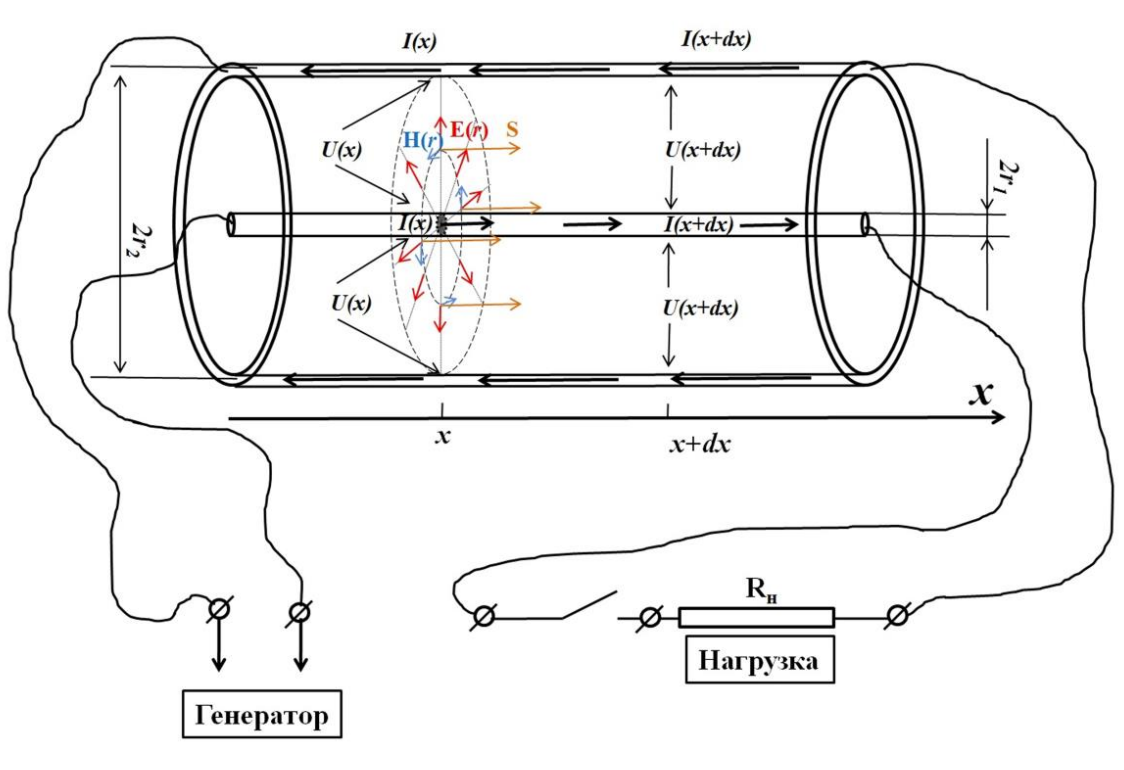
\includegraphics[width=0.9\textwidth]{установка.png}
	\label{fig:boiler}
\end{figure}

Соберем данную установку.

\section{Измерения, Обработка}

\subsection{Часть I. Оценка фазовой и групповой скорости}

1) Согласованная нагрузка имеет сопротивление 50 Ом

2) С увеличением частоты амплитуда на выходе падает, меняется сдвиг фазы.

На входе амплитуда не меняется.

3) Резонансы наблюдаются на частотах

\begin{center}
\begin{tabular}{|c|c|}
\hline 
& $\nu$, МГц \\
\hline
$\nu_1$ & 3.97 \\
$\nu_2$ & 7.96 \\
$\nu_3$ & 11.96 \\
$\nu_4$ & 15.97 \\
$\nu_5$ & 19.98 \\
$\nu_6$ & 23.99 \\
$\nu_7$ & 28.00 \\
\hline
\end{tabular}
\end{center}

4) Разброс значений от среднего значения 4 МГц не превышает десятка кГц. Таким образом дисперсия отсутствует(не превышает 1$\%$)

Фазовая скорость по теоретической формуле

\begin{equation}
	v_\phi = \frac{2 \pi \Delta \nu}{\frac{2 \pi}{k}} = (2 \pm 0.02) \cdot 10^8 \text{м/c}
\end{equation}

5) Выставим сопротивление нагрузки 1 МОм(обрыв)

6) Качественно:

Меняется амплитуда обоих сигналов

Фаза меняется быстро при амплитуде входного сиглала около нуля на $\pi$.

Сумма амплитуд является инвариантом.

7) Резонансы наблюдаются на частотах

\begin{center}
\begin{tabular}{|c|c|}
\hline 
& $\nu$, МГц \\
\hline
$\nu_1$ & 4.0 \\
$\nu_2$ & 8.0 \\
$\nu_3$ & 12.0 \\
$\nu_4$ & 16.0 \\
$\nu_5$ & 20.0 \\
$\nu_6$ & 24.0 \\
$\nu_7$ & 28.1 \\
\hline
\end{tabular}
\end{center}

8) Разброс значений от среднего значения 4 МГц не превышает десятка кГц. Таким образом дисперсия отсутствует(не превышает 1$\%$)

Фазовая скорость по теоретической формуле

\begin{equation}
	v_\phi = \frac{2 \pi \Delta \nu}{\frac{2 \pi}{k}} = (2 \pm 0.02) \cdot 10^8 \text{м/c}
\end{equation}

\subsection{Прямоугольные импульсы (согласованная линия)}

1-3) Выставим сопротивление нагрузки 50 Ом(согласованная нагрузка)

4) Качественно:

По одному входному и выходному импульсу покоятся(свойство развертки)

Остальные сжимаются к ним как к аттрактору при повышении частоты

Амплитуды импульсов не меняются.

5) Резонансы наблюдаются на частотах

\begin{center}
\begin{tabular}{|c|c|}
\hline 
& $\nu$, МГц \\
\hline
$\nu_1$ & 4.01 \\
$\nu_2$ & 8.02 \\
$\nu_3$ & 12.03 \\
$\nu_4$ & 16.04 \\
$\nu_5$ & 20.05 \\
\hline
\end{tabular}
\end{center}

6) Разброс значений от среднего значения 4 МГц не превышает десятка кГц. Таким образом дисперсия отсутствует(не превышает 1$\%$)

Фазовая скорость по теоретической формуле

\begin{equation}
	v_\phi = \frac{2 \pi \Delta \nu}{\frac{2 \pi}{k}} = (2 \pm 0.02) \cdot 10^8 \text{м/c}
\end{equation}

7) Выставим сопротивление нагрузки 1 МОм(обрыв)

8) От входного импульса образуется гаснущая отраженная волна, сдвинутая на $\pi$ относительно него.

Амплитуды сигналов суммируются.

9) Резонансы наблюдаются на частотах

\begin{center}
\begin{tabular}{|c|c|}
\hline 
& $\nu$, МГц \\
\hline
$\nu_1$ & 4.02 \\
$\nu_2$ & 8.04 \\
$\nu_3$ & 12.06 \\
$\nu_4$ & 16.08 \\
$\nu_5$ & 20.10 \\
\hline
\end{tabular}
\end{center}

10) Разброс значений от среднего значения 4 МГц не превышает десятка кГц. Таким образом дисперсия отсутствует(не превышает 1$\%$)

Фазовая скорость по теоретической формуле

\begin{equation}
	v_\phi = \frac{2 \pi \Delta \nu}{\frac{2 \pi}{k}} = (2 \pm 0.02) \cdot 10^8 \text{м/c}
\end{equation}

\subsection{Часть II. Амплитудно-частотная и фазово-частотная характеристики}

1-4) Выставим сопротивление нагрузки 50 Ом(согласованная нагрузка)

5) Снятые данные приведены в таблицах, построим соотвествующие графики

\newpage

\begin{center}
	\Large АЧХ
\end{center}

\begin{figure}[!h]
	\centering
	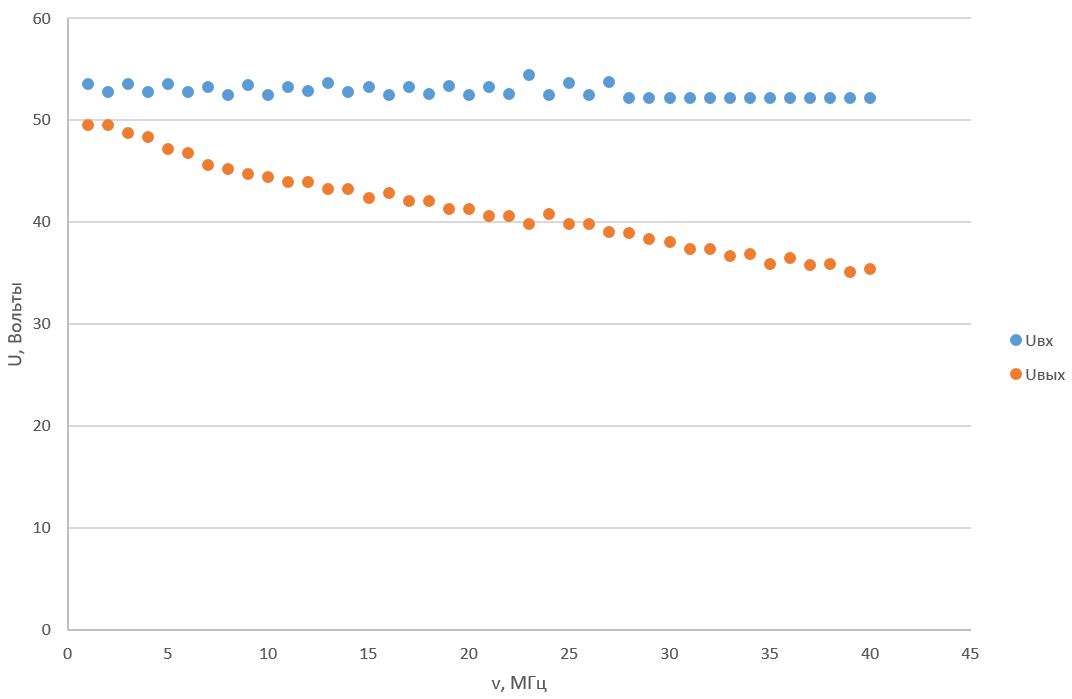
\includegraphics[width=0.9\textwidth]{ачх.png}
	\label{fig:boiler}
\end{figure}

\begin{center}
	\Large ФЧХ
\end{center}

\begin{figure}[!h]
	\centering
	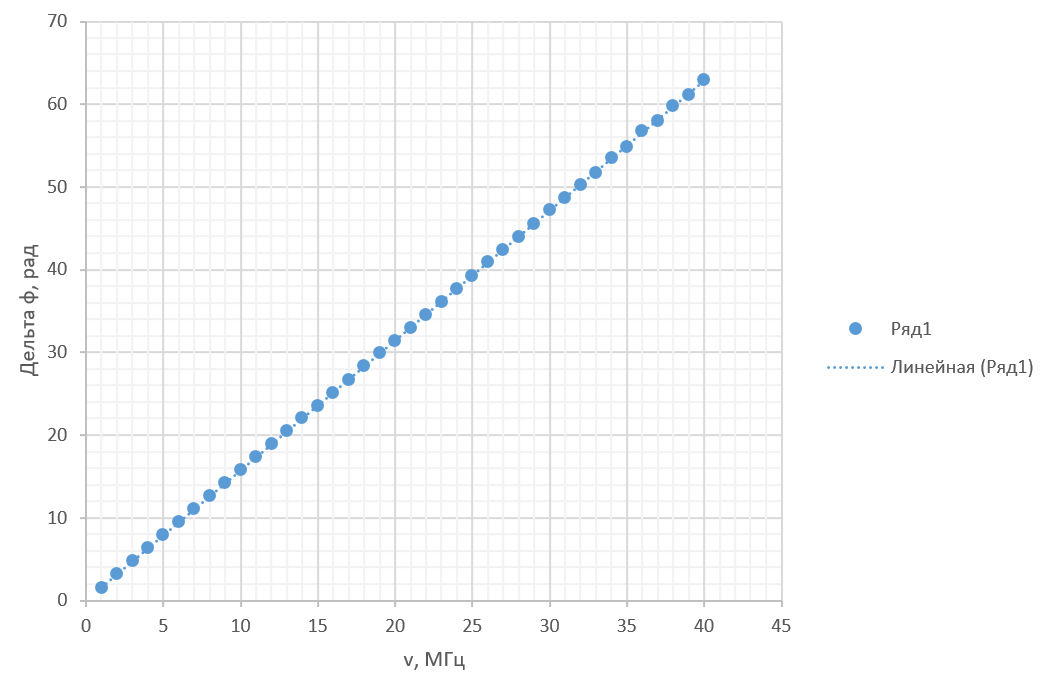
\includegraphics[width=0.9\textwidth]{фчх.png}
	\label{fig:boiler}
\end{figure}

\newpage

\subsection{Обработка. Часть I. Определение параметров коаксиального кабеля.}

Для определения характеристик коаксиального кабеля первое уравнение системы (22) с учётом (23) удобно переписать следующим образом

\begin{equation}
	y_1 = \frac{L_x C_x}{c^2} x_1
\end{equation}

\begin{equation}
	x_1 = \omega^2
\end{equation}

\begin{equation}
	y_1 = k(\omega)^2 - \alpha (\omega)^2
\end{equation}

Построим график y(x)

\begin{figure}[!h]
	\centering
	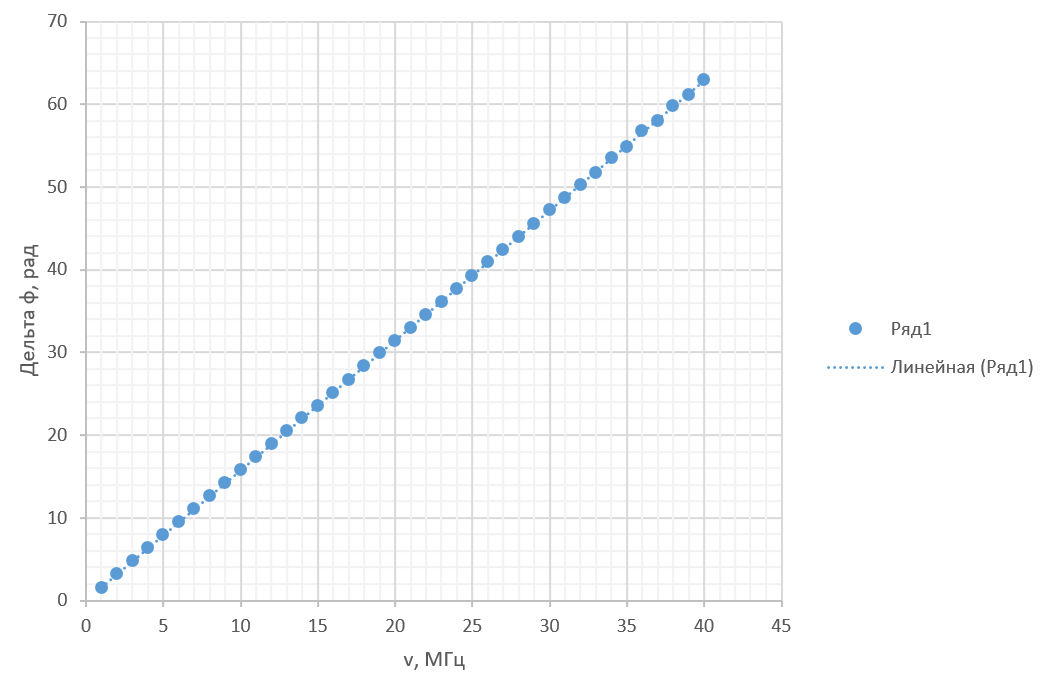
\includegraphics[width=0.9\textwidth]{фчх.png}
	\label{fig:boiler}
\end{figure}

Найдем угловые коэффициенты прямых для каждой установки по МНК.

\[
	a = \frac{<x_i y_i> - < x > < y_i >}{< x_i^2> - < x_i >^2}
\]

\[
	b = < \nu_i > - a < N_i >
\]

Также рассчитаем их погрешности

\begin{equation}
	S_a^2 = \frac{< x_i^2>}{< x_i^2 > - < x_i >^2} \cdot \frac{<  b_i - b > ^2}{n - 2}
\end{equation}

\begin{equation}
	y_1 = (3.4 \pm 6.3) \cdot 10^{-8} + (2.4996 \pm 0.0022) \cdot 10^{-21} \cdot x_1
\end{equation}

Тогда

\begin{equation}
	L_x C_x = (2.247 \pm 0.002) \text{ [СГС]}
\end{equation}

Наконец, с учетом $\frac{L_x}{C_x} = 2.5 \cdot 10^{21}$ [СГС], получим

\begin{equation}
	L_x = 2.500 \pm 0.001 \text{ см}
\end{equation}

\begin{equation}
	C_x = 0.89877 \pm 0.0004 \text{ см}
\end{equation}

Магнитная восприимчивость

\begin{equation}
	\mu = \frac{L_x}{2 ln(r_2 / r_1)} = \frac{C}{2 ln(11 / 4)} = 1.2357 \pm 0.005
\end{equation}

Диэлектрическая проницаемость же

\begin{equation}
	\epsilon = 2 C_x ln(r_2/r_1)  = 1.81839 \pm 0.0008
\end{equation}

Как видно, значения очень похожи на реальные

\subsection{Часть II. Определение удельной проводимости проводников. Метод А}

Из (23) и (28) следует:
$$
\alpha(\omega)=\frac{1}{l} \ln \left(\frac{U_0}{U_w}\right)=R_x C_x \frac{V_\phi}{2} .
$$
Если взять удельную проводимость для меди и подставить в известное выражение для характерной толщины скнн-слоя:
$$
\delta=\frac{c}{2 \pi \sqrt{\nu \sigma}},
$$
то окажется, что даже при минимальной частоте $v=1 \mathrm{MГц} \mathrm{эта} \mathrm{толшнна} \mathrm{будет} \mathrm{равна} \mathrm{около}$ 65 мкм, что прнмерно в десять раз меньше раднуса центрального проводника (днаметр центральной жилы равен $d=1,37 \mathrm{mM}$ ). Прн больших частотах характерная толшнна скннслоя ещё меньше. Поэтому для упрощення будем предполагать, что весь ток сосредоточен в прнповерхностном слое и потери, связанные с джоулевым нагревом опнсываются следуюшим выраженнем:
$$
d N=\left.\sigma E_0^2 \int_0^{\infty} e^{-2 \frac{z}{\delta}} d z d x L\right|_{L=\pi d}=\left.\sigma E_0^2 \cdot d x \cdot \pi d \cdot \frac{\delta}{2}\left(-e^{-2 \frac{z}{\delta}}\right)\right|_0 ^{\infty} \frac{\sigma \cdot \pi d}{d x} \cdot \frac{\delta}{2}(d U)^2=\frac{(d U)^2}{d R},
$$
где
$$
d R=\frac{d x}{\sigma \cdot \pi d} \cdot \frac{2}{\delta}
$$
Погонное сопротивленне с учётом скин-эффекта можно определить следующнм образом:
$$
R_x=\frac{d R}{d x}=\frac{2}{\sigma \cdot \pi d \cdot \delta} .
$$
Или, с учётом выражения для характерной толшнны скин-слоя (34), имеем:
$$
R_x=\frac{4 \sqrt{\nu}}{\sqrt{\sigma} \cdot c \cdot d} .
$$
Таким образом, подставляя (38) в (33) приходим к зависимости:
$$
\alpha(\omega)=\frac{1}{l} \ln \left(\frac{U_0}{U_\mu}\right)=\frac{4}{\sqrt{\sigma} \cdot d} C_x \frac{V_\phi}{c} \sqrt{v} .
$$
Это выражение можно переписать в следующем виде:
$$
y_2=\frac{4}{\sqrt{\sigma} \cdot d} C_x \frac{V_\phi}{c} x_2,
$$
где
$$
\begin{aligned}
& x_2=\sqrt{v}, \\
& y_2=\alpha(\omega) .
\end{aligned}
$$

\newpage

Построим график $a(\omega)$ от $\nu$

\begin{figure}[!h]
	\centering
	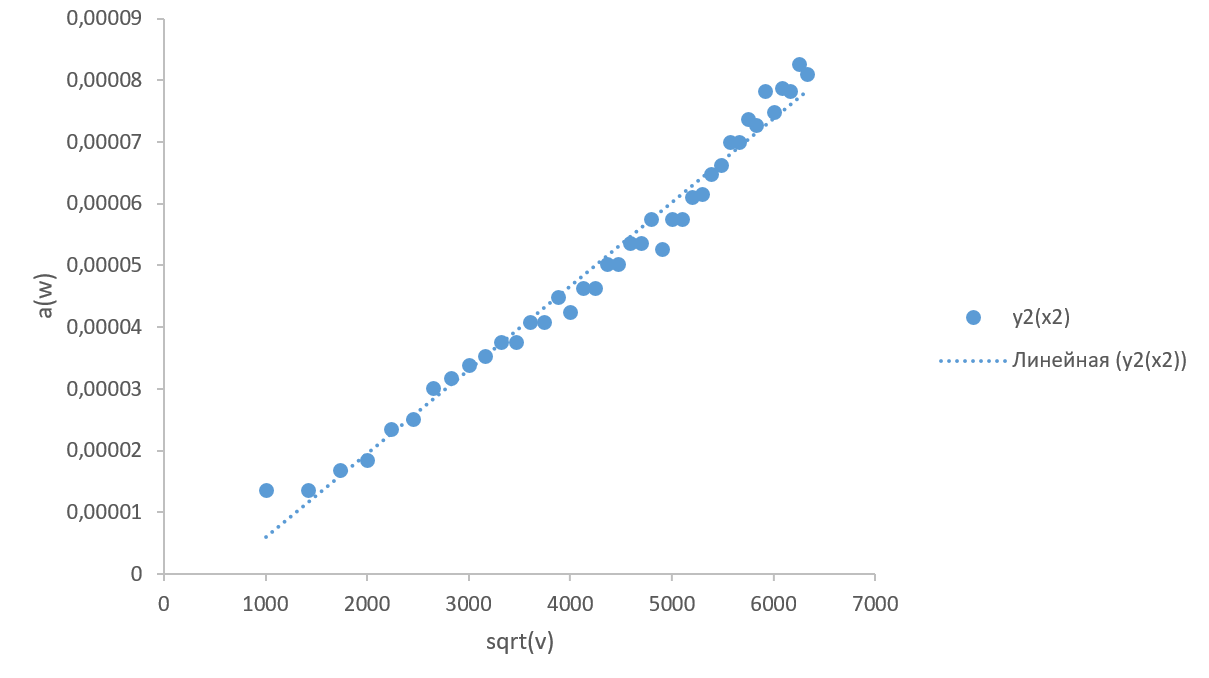
\includegraphics[width=0.9\textwidth]{граф2.png}
	\label{fig:boiler}
\end{figure}

Найдем угловые коэффициенты прямых для каждой установки по МНК.

\[
	a = \frac{<x_i y_i> - < x > < y_i >}{< x_i^2> - < x_i >^2}
\]

\[
	b = < \nu_i > - a < N_i >
\]

Также рассчитаем их погрешности

\begin{equation}
	S_a^2 = \frac{< x_i^2>}{< x_i^2 > - < x_i >^2} \cdot \frac{<  b_i - b > ^2}{n - 2}
\end{equation}

\begin{equation}
	y_1 = (-7.6 \pm 1.4) \cdot 10^{-6} + (1.358 \pm 0.031) \cdot 10^{-8} \cdot x
\end{equation}

По наклону прямой на графике, можно определить удельную проводимость $\sigma$
$$
\sigma=\left(\frac{4 C_x V_\phi}{c \cdot d \cdot\left(\Delta y_2 / \Delta x_2\right)}\right)^2 = (1.66 \pm 0.08) \cdot 10^{18} \text{ [СГС]}
$$

Значение проводимости близко к табличному значению ($1.54 \cdot 10^{18}$)

\subsection{Метод Б}

Подставив выражение для $\gamma$ из (14) во второе уравнение системы (22) и сокращая на квадрат скорости $V_\phi^2$ легко прнйти к выражению:
$$
2 \alpha k=\omega R_x C_x .
$$
(44)
Зная амплитуду колебаний и сдвиг фазы в конце длинной линии относительно входного сигнала экспериментально можно определнть как $\alpha(\omega)$, так и $k(\omega)$ (см., например, выражения (28) и (29)). Таким образом, выражение (44) можно представить в следующем виде:
$$
y_3=\frac{4 \pi \cdot C_x}{\sqrt{\sigma} \cdot d \cdot c} x_3,
$$
где
$$
x_3=v^{3 / 2},
$$
$$
y_3=\alpha(\omega) \cdot k(\omega)=\frac{1}{l} \ln \left(\frac{U_0}{U_n}\right) \cdot \frac{\Delta \varphi}{l} .
$$

Построим зависимость $y_3$ от $x_3$.

\begin{figure}[!h]
	\centering
	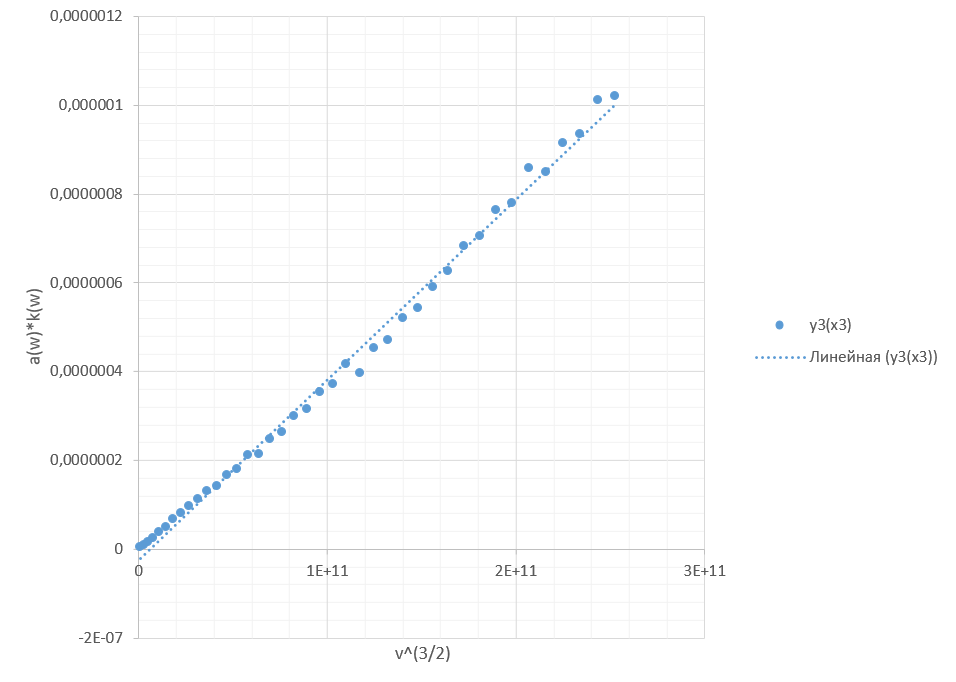
\includegraphics[width=0.9\textwidth]{граф3.png}
	\label{fig:boiler}
\end{figure}


\begin{equation}
	y_3 = (-2.57 \pm 0.6) \cdot 10^{-8} + (4.058 \pm 0.046)\cdot 10^{-18}\cdot x
\end{equation}

По наклону, полученной прямой определим удельную проводнмость $\sigma$

$$
\sigma=\left(\frac{4 \pi \cdot C_x}{d \cdot c\left(\Delta y_3 / \Delta x_3\right)}\right)^2 = 1.84 \pm 0.04 \cdot 10^{18} \text{ [СГС]}
$$

\subsection{Длинная линия. Модель}

\newpage

1) Соберем схему как на рисунке

\begin{figure}[!h]
	\centering
	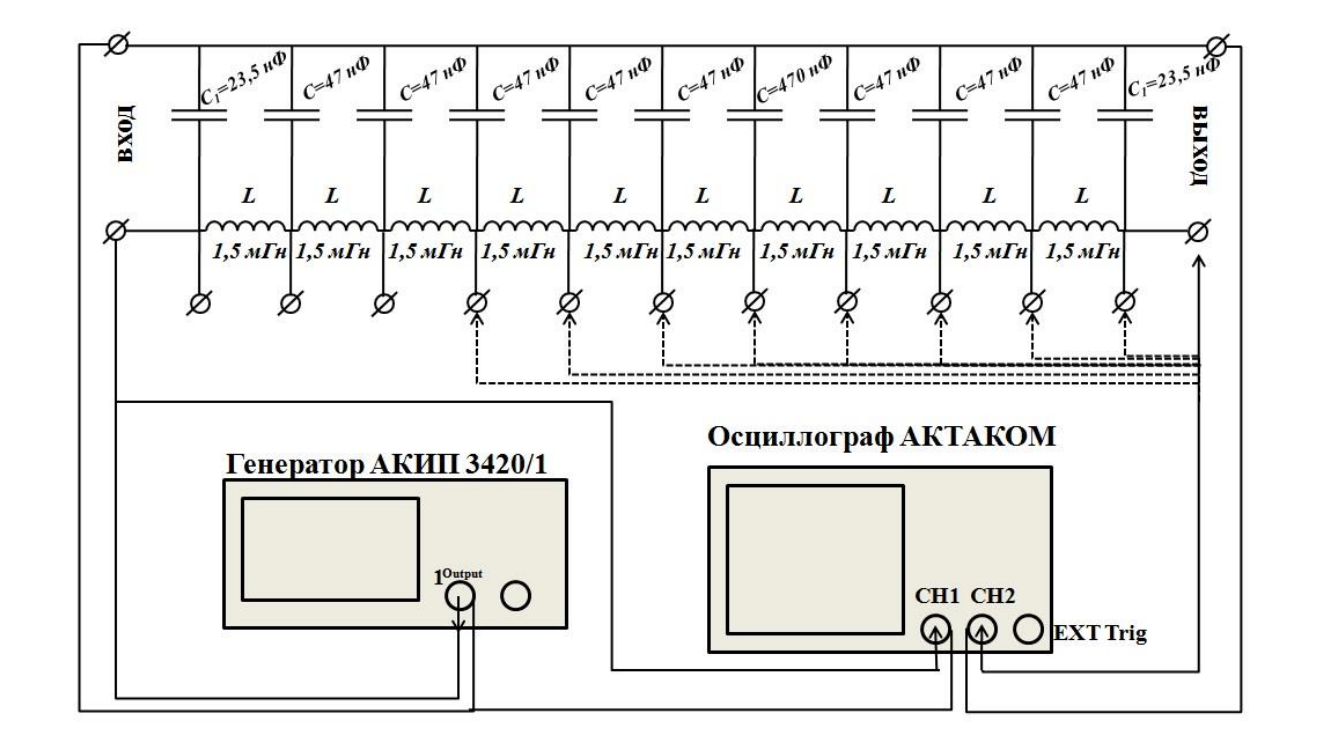
\includegraphics[width=0.9\textwidth]{установка2.png}
	\label{fig:boiler}
\end{figure}

Придельная частота распространения сигнала для установки

\begin{equation}
	\nu_0 = \frac{1}{\pi \sqrt{L C}} = 37.9 \text{ кГц}
\end{equation}

Согласованная нагрузка для цепи

\begin{equation}
	R_0 = \sqrt{\frac{L}{C}} = 178.6 \text{ Ом}
\end{equation}

2) Убедимся, что согласующее сопротивление подходящее

3, 7) Замерим сдвиг фаз в зависимости от частоты и построим график $\phi(\nu)$.

\begin{figure}[!h]
	\centering
	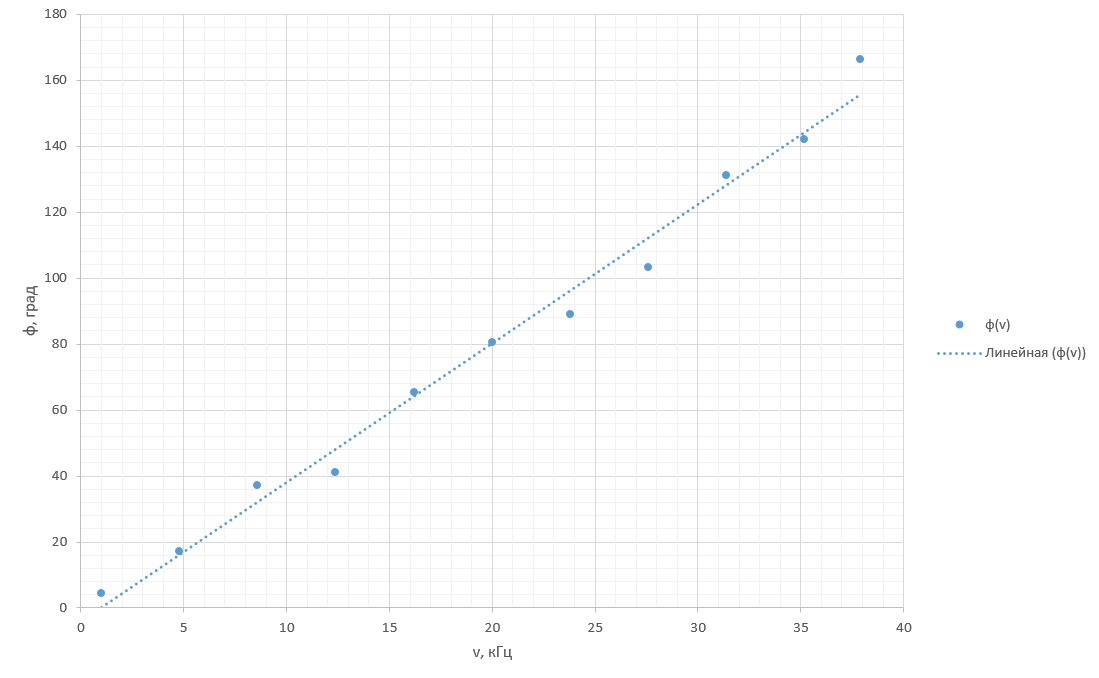
\includegraphics[width=0.9\textwidth]{граф4.png}
	\label{fig:boiler}
\end{figure}

Линейная зависимость полностью согласуется с теорией

\begin{equation}
	\Delta \phi = \frac{2 \pi \nu l}{v_\phi}
\end{equation}

4) Таблица резонансных частот при согласованной нагрузке

\begin{center}
\begin{tabular}{|c|c|}
\hline 
& $\nu$, кГц \\
\hline
$\nu_1$ & 4.2 \\
$\nu_2$ & 8.0 \\
$\nu_3$ & 13.0 \\
$\nu_4$ & 17.7 \\
$\nu_5$ & 21.2 \\
$\nu_6$ & 25.8 \\
\hline
\end{tabular}
\end{center}

При разрыве цепи же

\begin{center}
\begin{tabular}{|c|c|}
\hline 
& $\nu$, кГц \\
\hline
$\nu_1$ & 5.4 \\
$\nu_2$ & 7.8 \\
$\nu_3$ & 9.7 \\
$\nu_4$ & 14.6 \\
$\nu_5$ & 19.0 \\
$\nu_6$ & 23.3 \\
$\nu_7$ & 26.9 \\
\hline
\end{tabular}
\end{center}

5) Построим соответствующие графики

\newpage

\begin{figure}[!h]
	\centering
	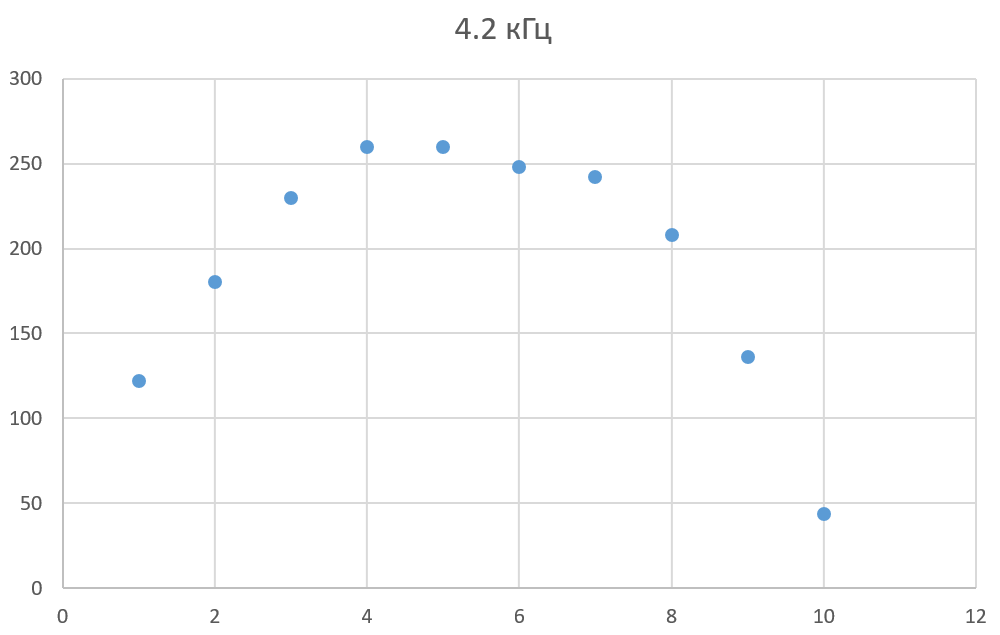
\includegraphics[width=0.9\textwidth]{1.png}
	\label{fig:boiler}
\end{figure}

\begin{figure}[!h]
	\centering
	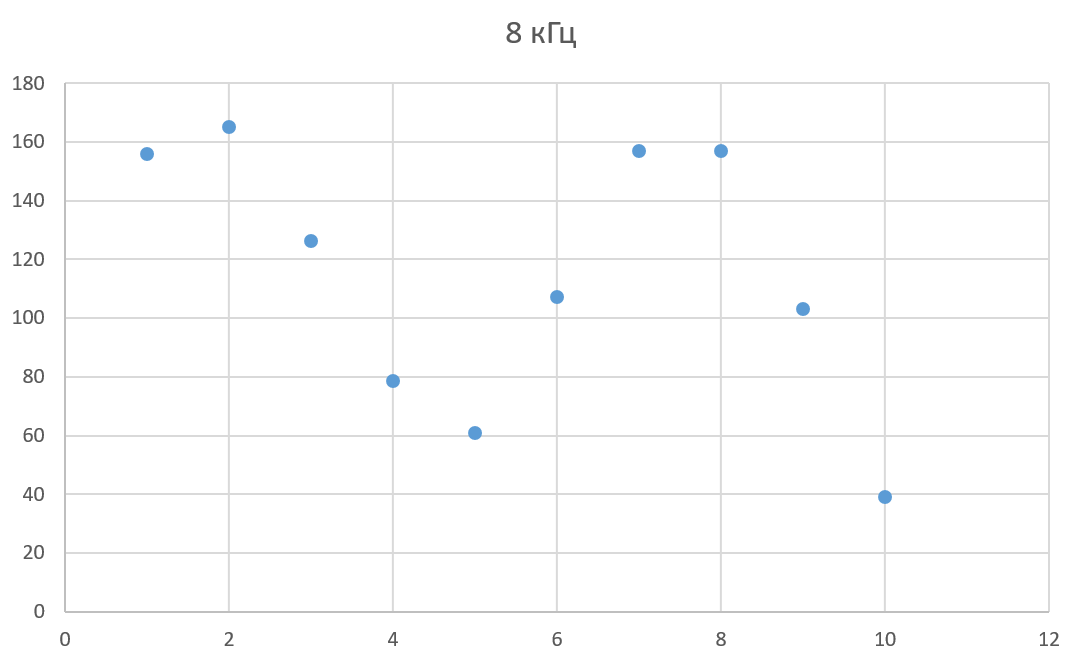
\includegraphics[width=0.9\textwidth]{2.png}
	\label{fig:boiler}
\end{figure}

\newpage

\begin{figure}[!h]
	\centering
	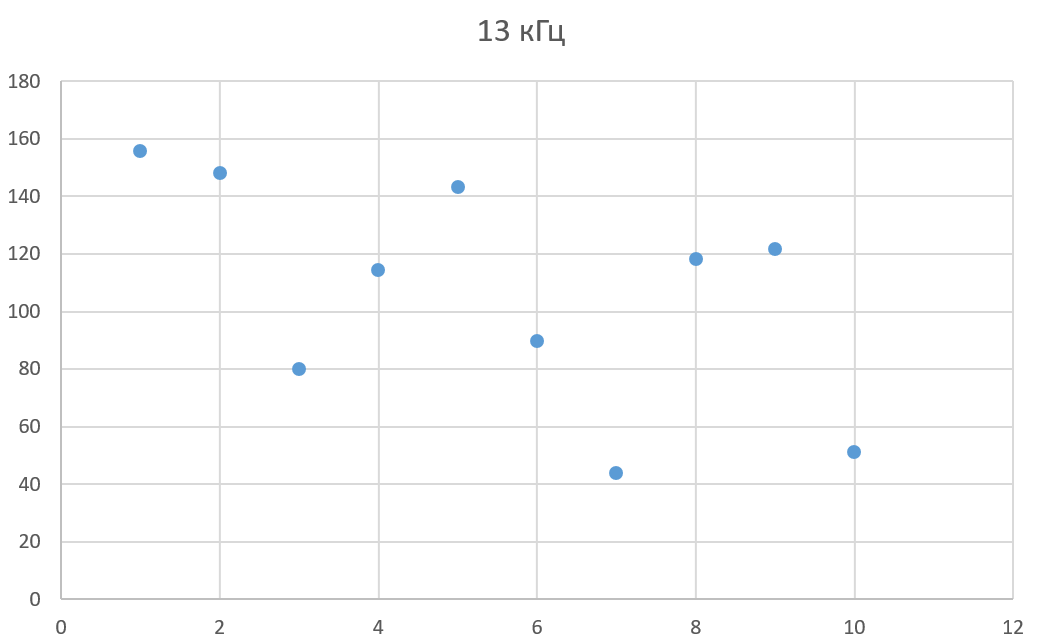
\includegraphics[width=0.9\textwidth]{3.png}
	\label{fig:boiler}
\end{figure}

\begin{figure}[!h]
	\centering
	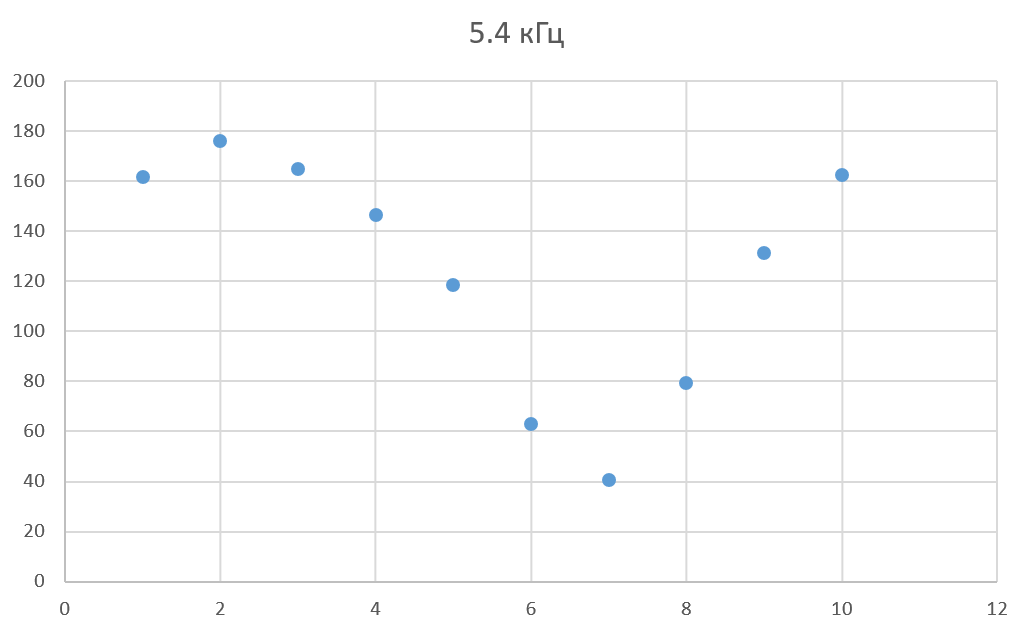
\includegraphics[width=0.9\textwidth]{4.png}
	\label{fig:boiler}
\end{figure}

\newpage

\begin{figure}[!h]
	\centering
	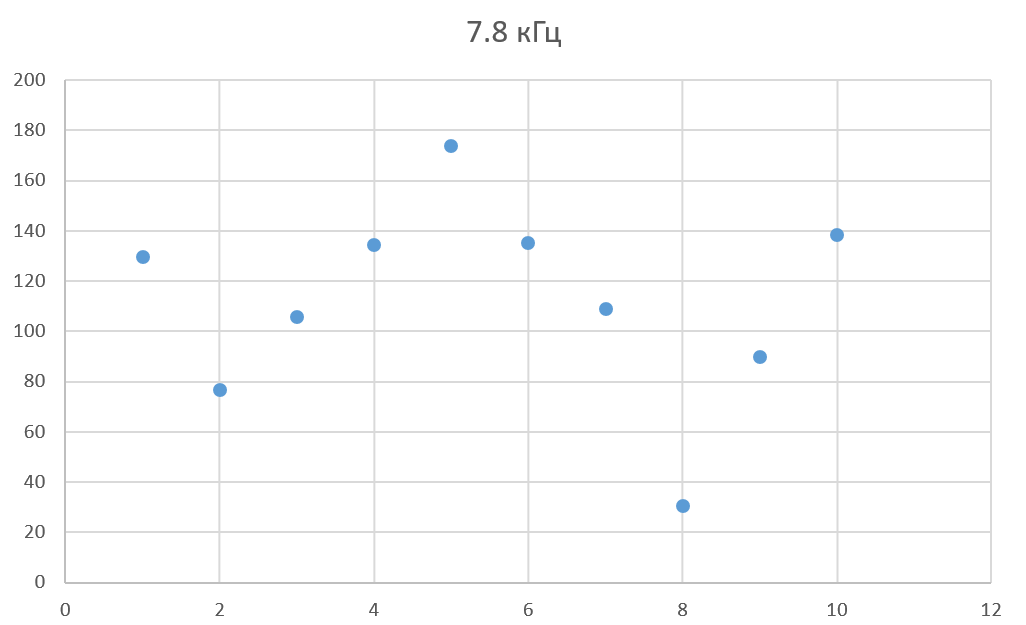
\includegraphics[width=0.9\textwidth]{5.png}
	\label{fig:boiler}
\end{figure}

\begin{figure}[!h]
	\centering
	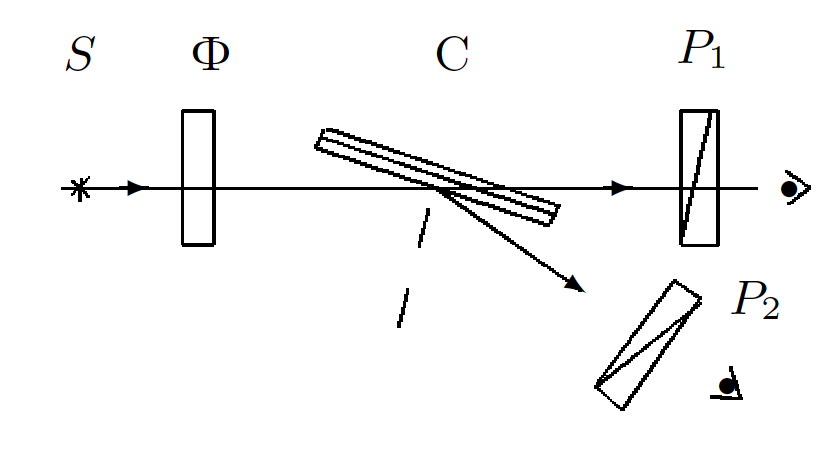
\includegraphics[width=0.9\textwidth]{6.png}
	\label{fig:boiler}
\end{figure}

\newpage

На графиках можно наблюдать пространственное распределение амплитуды колебаний точек волны, соответствующее стоячей волне в цепи. Диаграммы обрыва цепи сдвинуты на $\pi$ по фазе относительно согласованной нагрузки. На графиках хорошо прослеживается синусоидальная форма сигнала.

\section{Вывод}

Лабораторная работа фактически подтвердила применимость волнового уравнения для систем различного сорта, с достаточно высокой точностью.

\section{Ресурсы}

Расчет по МНК: метод-наименьших-квадратов.рф


\end{problem}
\end{document}